
\chapter{Two-dimensional Numerical Integration}
\label{sec:integrale}

This chapter is devoted to the numerical computation of integrals of
the type
\begin{equation}
  \label{eq:integral:to:compute}
  \int_{\check{A}\oplus B} \aire(A\,\cap\,(B-t)) \,\phi(t)
  \,dt,
\end{equation}
where $A$ and $B$ are bounded polygons and $\phi$ is an arbitrary
integrable dispersal function. As seen in
Chapter~\ref{sec:geom:algo}, without loss of generality we can focus
on the case when both $A$ and $B$ are convex.

We will start by preliminary remarks concerning the smoothness of the
integrand. Then we will discuss two methods for numerical integration:
\begin{itemize}
\item A simple randomized discretization of the integral;
\item An adaptive cubature method.
\end{itemize}

The first method, described in Section~\ref{sec:integration:autres},
combines simple discretization and Monte-Carlo techniques. This method
is quite robust (convergence even for non-smooth integrands). It
yields unbiased estimates and it is able to assess its precision.
However it may be slow compared to other methods.

The second method consists of an adaptive cubature. First, the domain of
integration (a convex polygon) is triangulated. Then the integral over
each triangle is approximated using the adaptive cubature method
proposed by Berntsen and Espelid~\cite{berntsen_espelid}. The
convergence of this method depends on the smoothness of the
integrand. It may fail to converge if the integrand cannot be
approximated locally by a polynomial. Some basic results about the
smoothness of the integrand in Equation~\eqref{eq:integral:to:compute}
are stated in Section~\ref{sec:regularite}. Details about the
adaptive cubature method are provided in Section~\ref{sec:cubature}.


\section{Smoothness of the integrand}
\label{sec:regularite}

The integrand in Equation~\eqref{eq:integral:to:compute} is the
product of two functions:
\begin{equation*}
  \aire(A\,\cap\,(B-t)) \text{ and } \phi(t).
\end{equation*}
The function $t\mapsto\aire(A\,\cap\,(B-t))$ is a piecewise linear
function. Its support $\check{A}\oplus B$ can be split by line
segments obtained by adding edges of $\check{A}$ and edges of $B$, see
Figure~\ref{fig:partition:minkowski}. Inside each cell of this
partition, $t\mapsto\aire(A\,\cap\,(B-t))$ behaves linearly. The
differential $t\mapsto\aire(A\,\cap\,(B-t))$ is not continuous along
the network of cell boundaries.
\begin{figure}[htbp]
  \centering
  \input{VignetteDir/graphics/div_minkowski_convexe.pstex_t}
  \caption{Partitionning of the Minkowski sum of two convex polygons
    $A$ and $B$ according to their edges.}
  \label{fig:partition:minkowski}
\end{figure}

The smoothness of the whole integrand also depends on the smoothness
of the dispersal function $\phi$. For instance, the dispersal
function given in Equation~\eqref{eq:dispersion:colbach} is infinitely
continuously differentiable except at the origin where it is not twice
differentiable.  Then the whole integrand is infinitely continuously
differentiable except along the cell boundaries in the partition of
the Minkowski sum where it is not differentiable and at the origin
where it is not twice differentiable. Another example: the dispersal
function given in Equation~\eqref{eq:dispersion:klein} is not
differentiable at the origin and it is not twice differentiable along
a circle with radius $1.5$ meter centered at the origin. Then the
whole integrand is not differentiable neither at the origin nor along
the cell boundaries and it is not twice differentiable along the circle.


\section{Method based on grids of points}
\label{sec:integration:autres}

A simple and intuitive method to perform numerical integration consists
of evaluating the integrand over a regular grid of points. The integral
is then approximated by summing the integrand over the grid points, and
by multiplying the result by the volume of each cell in the grid.
Provided the grid position is randomised, this method yields an unbiased
estimate of the integral. In addition, it can be repeated
several times, with grid positions randomised independently. The
integral is then estimated by the mean over the replicated grids. Replications
increase precision but also allow the standard error to be estimated. 

To simplify, this method will be called \textbf{the grid method} in the
sequel. In \verb+CaliFloPP+, the distances between the nodes of the grids are the same
for all grids and they are chosen by the user. The number of
replications is also set by the user.

\label{grille}
Let $A$ and $B$ be two polygons. The main steps are~:
\begin{enumerate}
\item
calculation of the Minkowski sum $\check{A}\oplus B$~;
\item
determination of the smallest rectangle which includes the Minkowski sum
and whose sides are parallel to the axes (see Fig.~\ref{integrale})~;
\item
integration over this rectangle, with the integrand multiplied by a coefficient 
$w$ equal to~1 if the point is in the Minkowski sum, to~0 otherwise.
\end{enumerate}

Integration is performed as mentioned above, using several grids of
points with the following properties~:
\begin{itemize}
\item all grids have the same $x$ and $y$ lags between adjacent nodes, chosen
  by the user~;
\item each grid is positioned randomly on the integration area, by
  shifting it randomly relatively to the origin. The shifting is
  determined by pseudo-random numbers from the uniform distributions
  over the intervals $[0, p_x]$ and $[0, p_y]$, where $p_x$ and $p_y$
  denote the $x$ and $y$ lags between adjacent grid nodes.
\end{itemize}
The integral is estimated by the mean integral over the replicated grids.

\subsection{Additional results}
\begin{itemize}
\item
\textbf{Standard deviation}

The \texttt{standard deviation} is defined as~: 
\begin{equation}
\mathrm{sd} = \frac{ \sqrt{\sum_{i=1}^{r} (a_{i} - a_{\bullet})^2}} {
  r-1}
\end{equation}
where  $a_{i}$ is the integral value calculated by replication $i$,
and $r$ the number of grid replications.

\item\textbf{Coefficient de variation} 

The \texttt{coefficient de variation} is defined as~: 
\begin{equation}
\mathrm{CV} = \frac{\mathrm{sd}}{a_{\bullet}}
\end{equation}


\item
\textbf{Precision and confidence intervals}
\label{it:gridprec}

Precision and confidence intervals can be calculated by the user
from the replications results.
For example, when the number of replications is large enough and  the
distributions are symmetric, they can be calculated from the quantile
of the Student distribution.
The half-range $\mathrm{hr}$ of the confidence
interval, or the absolute precision, is then defined as~:
\begin{equation}
\mathrm{hr} =  \mathrm{sd} \times \frac{\mathrm{qt}(r-1, p)}{\sqrt{r}}
\end{equation}
where  $\mathrm{qt}(n,p)$ is the quantile for probability $p$ of the Student
distribution with $n$ degrees of freedom.
The relative precision is $\frac{hr}{a_{\bullet}}$.
\end{itemize}


\begin{figure}[htbp]
  \begin{center}
  \includegraphics[width=9cm]{VignetteDir/graphics/integrale.eps}
  \end{center}
  \caption{Minimal rectangle including the Minkowski sum and grid of
    points before random shifting}
  \label{integrale}
\end{figure}



\section{Adaptive cubature method}
\label{sec:cubature}

The cubature method over triangles DCUTRI \cite{berntsen_espelid} uses
an integration rule of degree $27$ based on $37$ points. Using
estimates of approximation errors, triangles are iteratively split
into subtriangles until a nominal error is reached. At each iteration
the triangle with the largest error is selected for further splitting.
The procedure is expected to converge if the integrand is smooth
enough inside each triangle. For instance, if the dispersal function
is singular at the origin and if the domain of integration
$\check{A}\oplus B$ contains the origin, one expects a quicker
convergence when the origin is a vertex of the triangulation. Hence
(see Figure~\ref{fig:triangulation:minkowski}):
\begin{itemize}
\item if $\check{A}\oplus B$ does not contain the origin, it is
  triangulated from an arbitrary vertex,
\item if $\check{A}\oplus B$ contains the origin $O$, it is
  triangulated from $O$.
\end{itemize}

\begin{figure}[htbp]
  \centering
  \input{VignetteDir/graphics/triangulation_minkowski.pstex_t}
  \caption{Triangulation of the Minkowski sum of two convex polygons
    $A$ and $B$. If $A$ and $B$ are disjoint (top), the Minkowski sum
    $\check{A}\oplus B$ does not contain the origin and is
    triangulated from an arbitrary vertex. If $A$ and $B$ share a
    common edge (middle) or if $A=B$ (bottom), the Minkowski sum
    $\check{A}\oplus B$ contains the origin $O$ and is
    triangulated from $O$.}
  \label{fig:triangulation:minkowski}
\end{figure}

A further refinement is to avoid to integrate over areas where the
dispersal function is considered as negligible that is below a chosen
threshold $r_\text{max}$. Note that whenever the dispersal function
is non-negative and tends to $0$ at infinity, it can be considered in
practice as null when it is less than the smallest positive number
greater than zero for the used type of number. Thus instead of
integrating over the whole Minkowski sum $\check{A}\oplus B$, one may
integrate only on its intersection with a disc centered at the origin
and with radius $r_\text{max}$. In practice it is simpler to replace
the disc by a regular polygon e.g.\ an octogon containing it, see
Figure~\ref{fig:reduc:minkowski}. Hence integration is still performed
on a convex polygon.
\begin{figure}[htbp]
  \centering
  \input{VignetteDir/graphics/reduc_minkowski.pstex_t}
  \caption{Reduction of the domain of integration. Beyond
    $r_\text{max}$ the dispersal function is considered as
    negligible. The integral is computed only over the intersection of
    $\check{A}\oplus B$ and an octogon (blue solid line) containing
    the disc centered at the origin with radius $r_\text{max}$ (blue
    dash line). Top: the Minkowsi sum $\check{A}\oplus B$ does not
    contain the origin
. Bottom: the Minkowski sum contains the origin.}
  \label{fig:reduc:minkowski}
\end{figure}

%%% On n'a plus besoin des graphiques octo.eps et octo0.eps




%%% Local Variables: 
%%% mode: latex
%%% TeX-master: "../manotice"
%%% End: 
